
A continuación, se describen algunos hechos estilizados sobre la dinámica de la violencia y la presencia de grupos armados en Colombia, derivados de información recopilada por el Ministerio de Defensa y la Fiscalía.
\\\\
La figura 1 muestra un mapa de los municipios de Colombia, distinguiendo entre los que no tienen presencia de grupos armados y aquellos que cuentan con al menos uno. Se observa que, de 2020 a 2023, aumenta el número de municipios con actores armados, sobre todo en zonas alejadas de los centros urbanos y en corredores estratégicos vinculados a economías ilegales.

\begin{figure}[h]
    \centering
    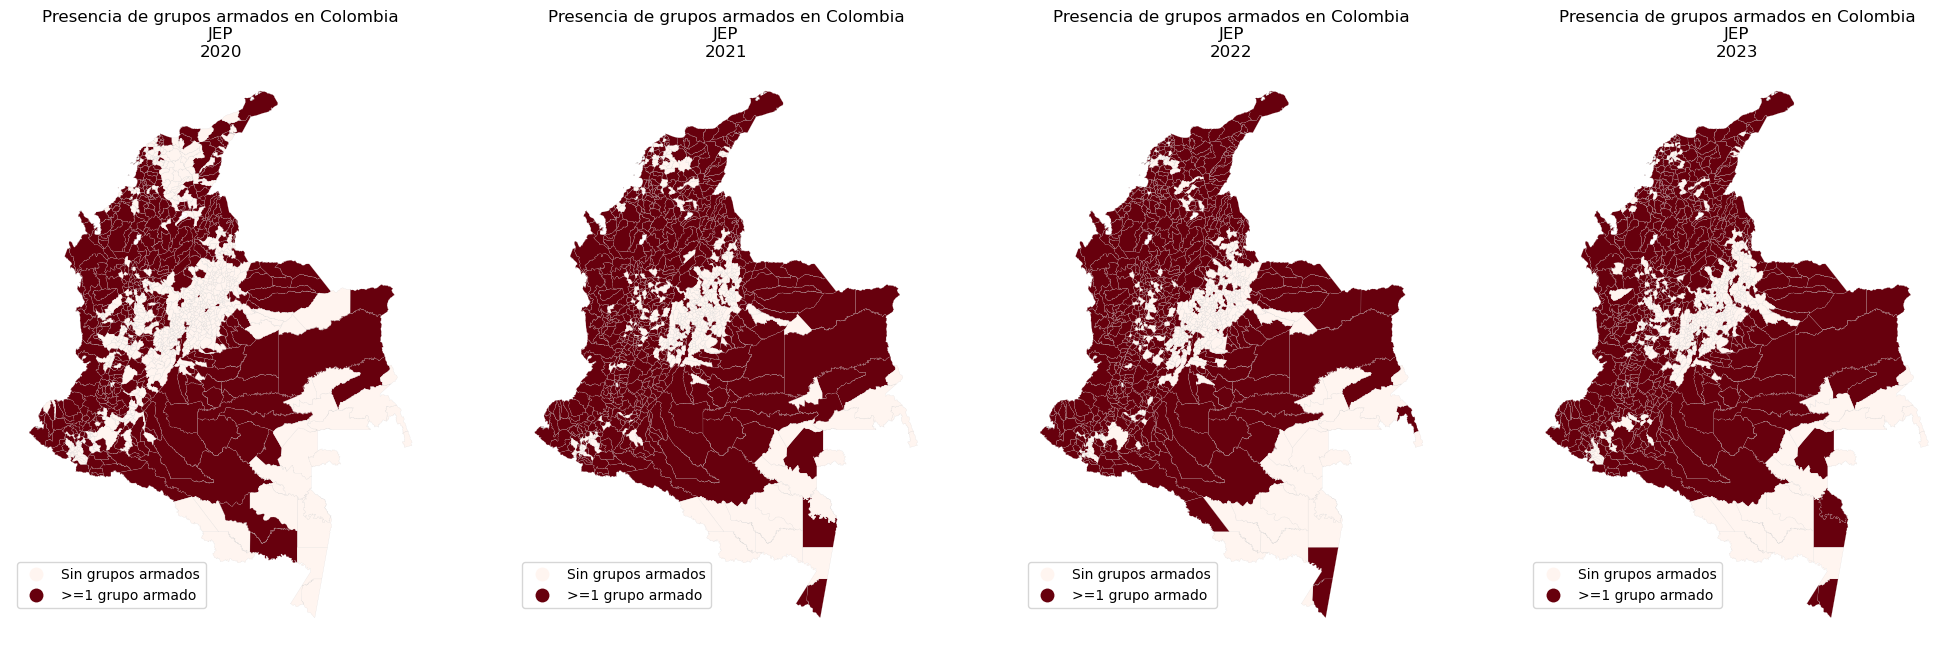
\includegraphics[width=0.8\textwidth]{Seminario de Tesis/Primera presentación/images/image.png}
    \caption{Clasificación binaria de los municipios según la presencia de grupos armados.}
    \label{fig:graph1}
\end{figure}
\\
En cambio, la figura 2 emplea un degradado de color para mostrar cuántos grupos armados hay en cada municipio, desde cero hasta tres al mismo tiempo. Los tonos rojos más intensos indican lugares con varios grupos, lo que refleja una dinámica de violencia más compleja y un mayor riesgo de enfrentamientos. Así, se puede observar la expansión y consolidación de las zonas conflictivas a lo largo del tiempo, evidenciando el incremento de la superposición de grupos en distintas áreas.

\begin{figure}[h]
    \centering
    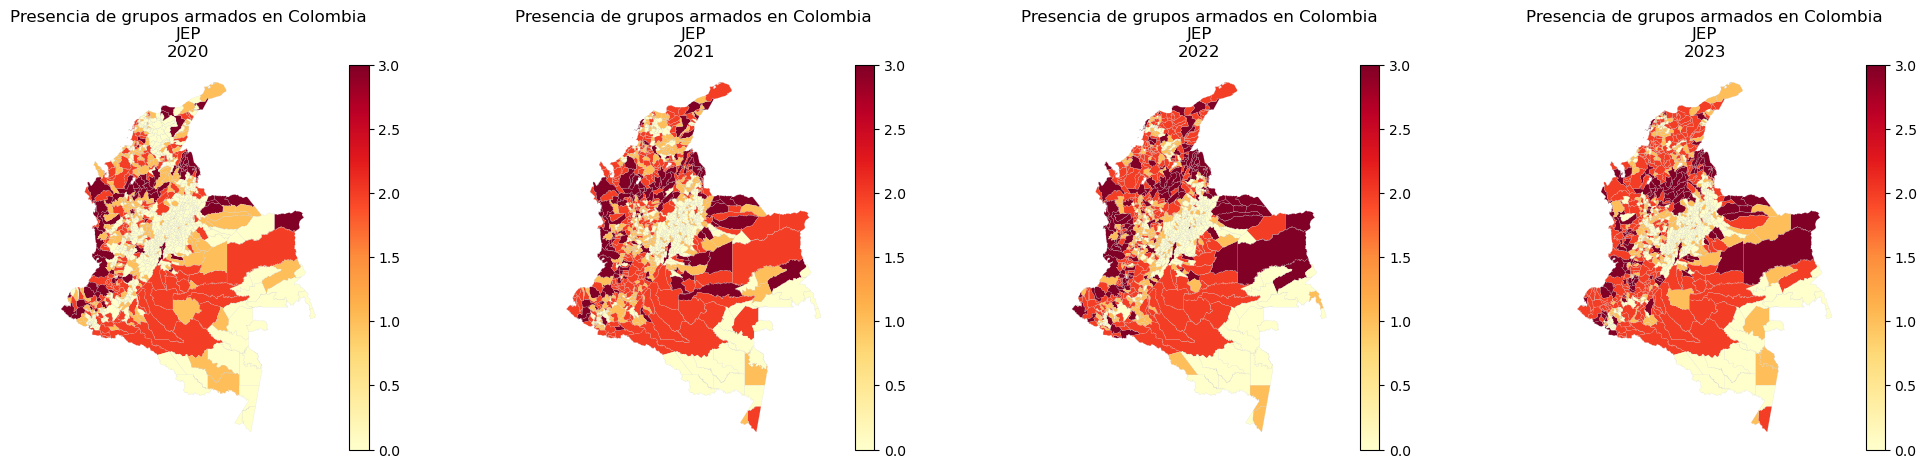
\includegraphics[width=0.8\textwidth]{Seminario de Tesis/Primera presentación/images/image 1.png}
    \caption{Concentración de grupos armados por municipio.}
    \label{fig:graph2}
\end{figure}
\\
Por su parte, la figura 3 muestra la evolución del IACV a lo largo del tiempo, comparando los datos de la Fiscalía General de la Nación y del Ministerio de Defensa Nacional. Se observa una tendencia en aumento desde 2020 hasta 2024, aunque con diferencias en la magnitud y variabilidad entre las dos fuentes. Esto sugiere que la expansión de grupos armados en Colombia a través de los años ha venido acompañado de un aumento agregado de la violencia en Colombia.
\\\\
\begin{figure}[h]
    \centering
    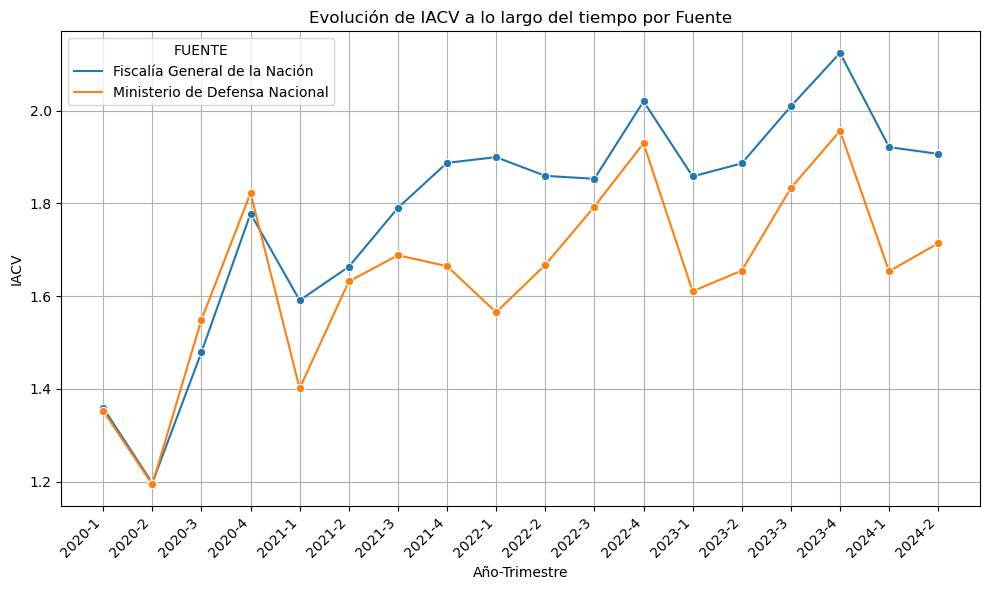
\includegraphics[width=0.8\textwidth]{Seminario de Tesis/Primera presentación/images/image 7.png}
    \caption{Evolución del IACV según los registros de la Fiscalía General de la Nación y el Ministerio de Defensa Nacional.}
    \label{fig:graph3}
\end{figure}

Asimismo, La figura 4 y 5 muestran la Curva de Lorenz del IACV para el año 2019 y 2024 respectivamente. Esta curva sirve para analizar cómo se reparte la violencia entre la población. Cuanto más se aleja la curva de la línea de igualdad perfecta (en rojo), mayor es la concentración en un grupo pequeño de la población. Para 2019, el índice de Gini es de 66\%, lo que indica que la violencia se concentra en pocos municipios. En contraste, para 2024, el índice de Gini sube a 73\%, reflejando que la concentración de la violencia es aún mayor. Así, en conjunto con los gráficos anteriores, se sugiere que este aumento de violencia, que ha sido acompañado de una expansión de grupos criminales en el país, no solo ha aumentado, si no que ha venido aumentando y concentrandose en una menor cantidad de municipios.
\newpage
\begin{figure}[h]
    \centering
    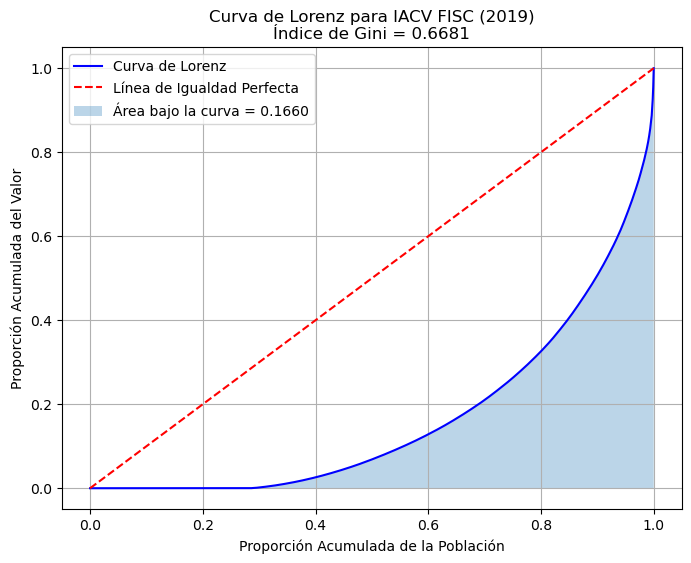
\includegraphics[width=0.7\textwidth]{Seminario de Tesis/Primera presentación/images/image 3.png}
    \caption{Curva de Lorenz del IACV para 2019.}
    \label{fig:graph4}
\end{figure}

\begin{figure}[h]
    \centering
    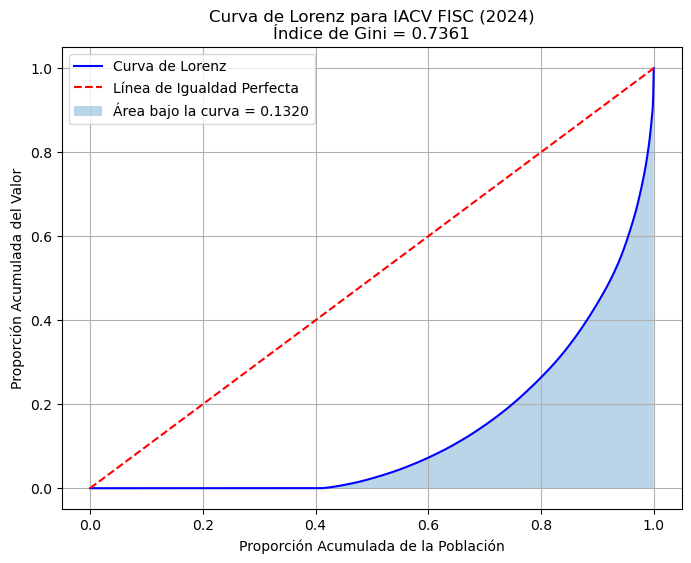
\includegraphics[width=0.7\textwidth]{Seminario de Tesis/Primera presentación/images/image 4.png}
    \caption{Curva de Lorenz del IACV para 2024.}
    \label{fig:graph5}
\end{figure}
\newpage
Para cerrar, la figura 6 y 7 muestran la relación entre los quintiles de variables asociadas al desarrollo y bienestar municipal y el valor medio del IACV, junto con sus intervalos de confianza al 95\%. 
\\\\
Para la figura 6 se utiliza como variable objetivo el índice de necesidades básicas insatisfechas. Se observa un incremento progresivo en el promedio del IACV entre los primeros cuatro quintiles, alcanzando su punto más alto en el cuarto. Por su parte, la figura 7 utiliza como variable objetivo el índice de alfabetización municipal. Se observa una disminución del promedio del IACV a partir del segundo quintil.
\\\\
Estos resultados indican que la violencia tiende a concentrarse en municipios con niveles de carencias elevados, pero no extremos. En los municipios con las mayores privaciones, quinto quintil en la figura 6 y primer quintil en la figura 7, el IACV presenta una ligera reducción. Asimismo, los intervalos de confianza evidencian la variabilidad de cada grupo y sugieren diferencias estadísticamente significativas.
\newpage
\begin{figure}[h]
    \centering
    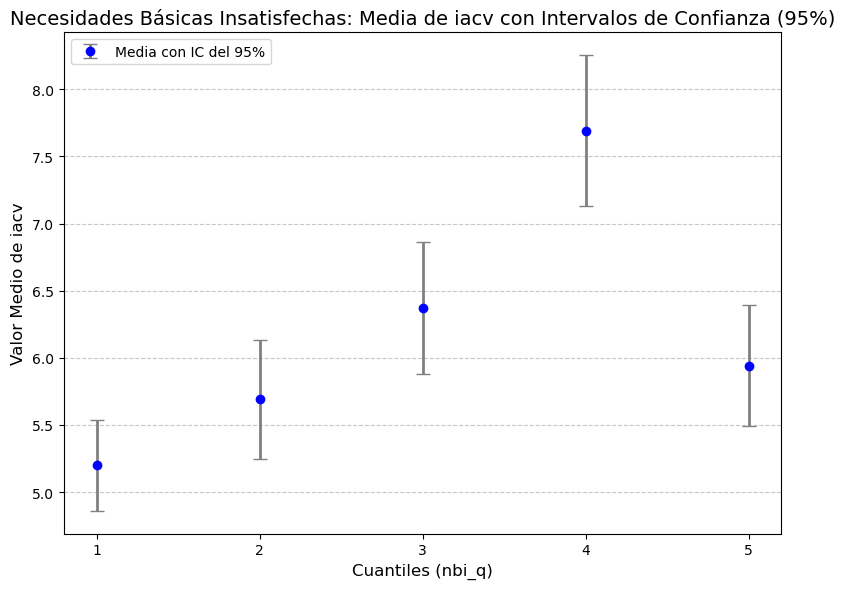
\includegraphics[width=0.7\textwidth]{Seminario de Tesis/Primera presentación/images/output1.png}
    \caption{Necesidades Básicas Insatisfechas vs. IACV con Intervalos de Confianza (95\%).}
    \label{fig:nbivia1}
\end{figure}
\begin{figure}[h]
    \centering
    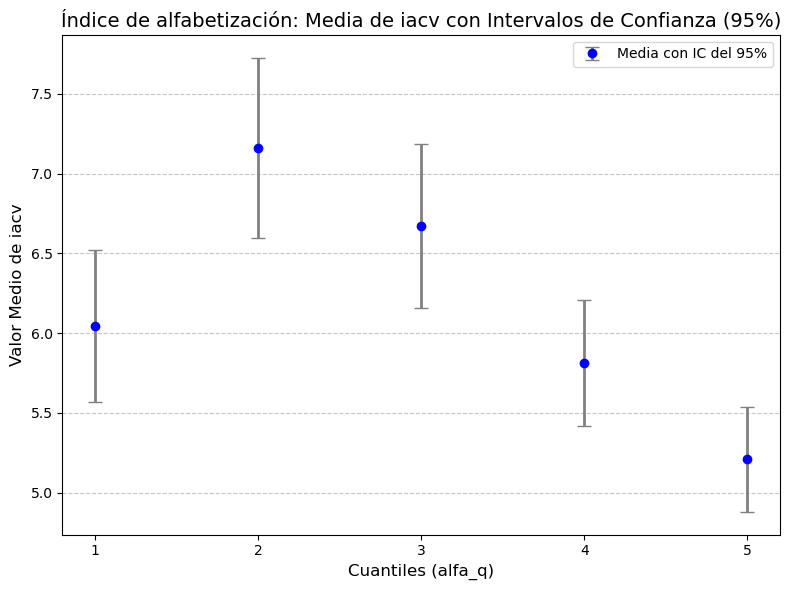
\includegraphics[width=0.7\textwidth]{Seminario de Tesis/Primera presentación/images/output2.png}
    \caption{Alfabetización vs. IACV con Intervalos de Confianza (95\%).}
    \label{fig:nbivia2}
\end{figure}

\newpage